\newcommand{\fileInfectorTagResultsAucTable}{
    \begin{table}[H]
        \centering
        \begin{tabular}{|p{2,8cm}||p{2,8cm} p{2,8cm} p{2,8cm}|}
            \hline
            File-infector Tag & ALOHA & Joint Embedding & Proposed Model \\
            \hline
            AUC-ROC & 0.597$\pm$0.108 & \textBF{0.682$\pm$0.100} & 0.603$\pm$0.098 \\
            \hline
        \end{tabular}
        \caption{AUC-ROC (Area Under Curve) of the different models for the \textbf{File-infector Tag} prediction task. Results were aggregated over \textBF{3} training runs with different weight initializations and minibatch orderings. Best results are shown in \textbf{bold}.} \label{tab:fileInfectorTag_auc}
    \end{table}
}

\newcommand{\fileInfectorTagResultsAtFprTable}{
    \begin{center}
        \begin{longtable}[c]{|p{3,2cm}||p{1,8cm} p{1,8cm} p{1,8cm} p{1,8cm} p{1,8cm}|}
            \hline
            File-infector Tag & \multicolumn{5}{c|}{{FPR}} \\
            & $10^{-5}$ & $10^{-4}$ & $10^{-3}$ & $10^{-2}$ & $10^{-1}$ \\
            \hline
            \endfirsthead

            \caption*{\raggedright ...continued from previous page} \\
            \hline
            File-infector Tag & \multicolumn{5}{c|}{\textbf{FPR}} \\
            & $10^{-5}$ & $10^{-4}$ & $10^{-3}$ & $10^{-2}$ & $10^{-1}$ \\
            \hline
            \endhead

            \caption*{\raggedleft ...continued on next page} \\
            \endfoot

            \caption{Mean and standard deviation results (TPR, Accuracy, Recall, Precision and F1-Score) of the different models for the \textbf{File-infector Tag} prediction task at different \textbf{FPR}s (\textit{False Positive Rates}). Results were aggregated over \textBF{3} training runs with different weight initializations and minibatch orderings. Best results are shown in \textbf{bold}. Under \textbf{TPR} results are also presented the percentage reduction in mean detection error and in ROC curve standard deviation introduced by the \textit{Proposed Model} with respect to both \textit{ALOHA} model and \textit{Joint Embedding}.} \label{tab:fileInfectorTag_results_at_fpr} \\
            \endlastfoot

            \multicolumn{6}{|c|}{\textbf{TPR}} \\
            \hline
            ALOHA & 0.023$\pm$0.026 & 0.023$\pm$0.026 & 0.023$\pm$0.026 & 0.108$\pm$0.104 & 0.160$\pm$0.147 \\
            Joint Embedding & \textBF{0.054$\pm$0.008} & \textBF{0.054$\pm$0.008} & \textBF{0.060$\pm$0.007} & \textBF{0.199$\pm$0.097} & \textBF{0.380$\pm$0.128} \\
            Proposed Model & 0.052$\pm$0.006 & 0.052$\pm$0.006 & 0.054$\pm$0.006 & 0.065$\pm$0.007 & 0.225$\pm$0.106 \\
            \hline
            Error Reduction wrt \newline ALOHA & 3.0\% & 3.0\% & 3.2\% & -4.8\% & 7.7\% \\
            Error Reduction wrt \newline Joint Embedding & -0.2\% & -0.2\% & -0.6\% & -16.7\% & -25.0\% \\
            \hline
            Std Reduction wrt \newline ALOHA & 76.9\% & 76.9\% & 76.9\% & 93.3\% & 27.9\% \\
            Std Reduction wrt \newline Joint Embedding & 25.0\% & 25.0\% & 14.3\% & 92.8\% & 17.2\% \\
            \hline
            \multicolumn{6}{|c|}{\textbf{Accuracy}} \\
            \hline
            ALOHA & 0.914$\pm$0.002 & 0.914$\pm$0.002 & 0.914$\pm$0.002 & 0.917$\pm$0.008 & 0.834$\pm$0.013 \\
            Joint Embedding & \textBF{0.916$\pm$0.001} & \textBF{0.916$\pm$0.001} & \textBF{0.916$\pm$0.001} & \textBF{0.920$\pm$0.009} & \textBF{0.854$\pm$0.012} \\
            Proposed Model & \textBF{0.916$\pm$0.001} & \textBF{0.916$\pm$0.001} & \textBF{0.916$\pm$0.001} & 0.908$\pm$0.001 & 0.844$\pm$0.012 \\
            \hline
            \multicolumn{6}{|c|}{\textbf{Recall}} \\
            \hline
            ALOHA & 0.023$\pm$0.026 & 0.023$\pm$0.026 & 0.023$\pm$0.026 & 0.108$\pm$0.104 & 0.160$\pm$0.147 \\
            Joint Embedding & \textBF{0.054$\pm$0.008} & \textBF{0.054$\pm$0.008} & \textBF{0.060$\pm$0.007} & \textBF{0.199$\pm$0.097} & \textBF{0.380$\pm$0.128} \\
            Proposed Model & 0.052$\pm$0.006 & 0.052$\pm$0.006 & 0.054$\pm$0.006 & 0.065$\pm$0.007 & 0.225$\pm$0.106 \\
            \hline
            \multicolumn{6}{|c|}{\textbf{Precision}} \\
            \hline
            ALOHA & \textBF{1.000$\pm$0.000} & \textBF{1.000$\pm$0.000} & \textBF{1.000$\pm$0.000} & 0.584$\pm$0.141 & 0.121$\pm$0.102 \\
            Joint Embedding & \textBF{1.000$\pm$0.000} & \textBF{1.000$\pm$0.000} & 0.888$\pm$0.027 & \textBF{0.610$\pm$0.151} & \textBF{0.262$\pm$0.064} \\
            Proposed Model & \textBF{1.000$\pm$0.000} & \textBF{1.000$\pm$0.000} & 0.974$\pm$0.036 & 0.388$\pm$0.031 & 0.179$\pm$0.076 \\
            \hline
            \multicolumn{6}{|c|}{\textbf{F1 Score}} \\
            \hline
            ALOHA & 0.044$\pm$0.049 & 0.044$\pm$0.049 & 0.044$\pm$0.049 & 0.170$\pm$0.155 & 0.138$\pm$0.121 \\
            Joint Embedding & \textBF{0.102$\pm$0.014} & \textBF{0.102$\pm$0.014} & \textBF{0.113$\pm$0.011} & \textBF{0.296$\pm$0.129} & \textBF{0.310$\pm$0.087} \\
            Proposed Model & 0.100$\pm$0.010 & 0.100$\pm$0.010 & 0.102$\pm$0.010 & 0.111$\pm$0.011 & 0.200$\pm$0.089 \\
            \hline
        \end{longtable}
    \end{center}
}

\newcommand{\fileInfectorTagResultsSummaryTable}{
    \begin{table}[H]
        \centering
        \begin{tabular}{|p{3,2cm}||p{1,8cm} p{1,8cm} p{1,8cm} p{1,8cm} p{1,8cm}|}
            \hline
            \multicolumn{6}{|c|}{File-infector Tag (at FPR $=1\%$)} \\
            \hline
            Model & TPR & Accuracy & Precision & Recall & F1 score \\
            \hline
            ALOHA & 0.108$\pm$0.104 & 0.917$\pm$0.008 & 0.584$\pm$0.141 & 0.108$\pm$0.104 & 0.170$\pm$0.155 \\
            Joint Embedding & \textBF{0.199$\pm$0.097} & \textBF{0.920$\pm$0.009} & \textBF{0.610$\pm$0.151} & \textBF{0.199$\pm$0.097} & \textBF{0.296$\pm$0.129} \\
            Proposed Model & 0.065$\pm$0.007 & 0.908$\pm$0.001 & 0.388$\pm$0.031 & 0.065$\pm$0.007 & 0.111$\pm$0.011 \\
            \hline
        \end{tabular}
        \caption{Summary of the mean and standard deviation results of the different models for the \textbf{File-infector Tag} prediction task at \textbf{FPR} $=1\%$. Results were aggregated over \textBF{3} training runs with different weight initializations and minibatch orderings. Best results are shown in \textbf{bold}.} \label{tab:fileInfectorTag_result_summary}
    \end{table}
}

\newcommand{\fileInfectorTagRocAloha}{
    \begin{figure}[H]
        \vspace*{-0.5cm}
        \centering
        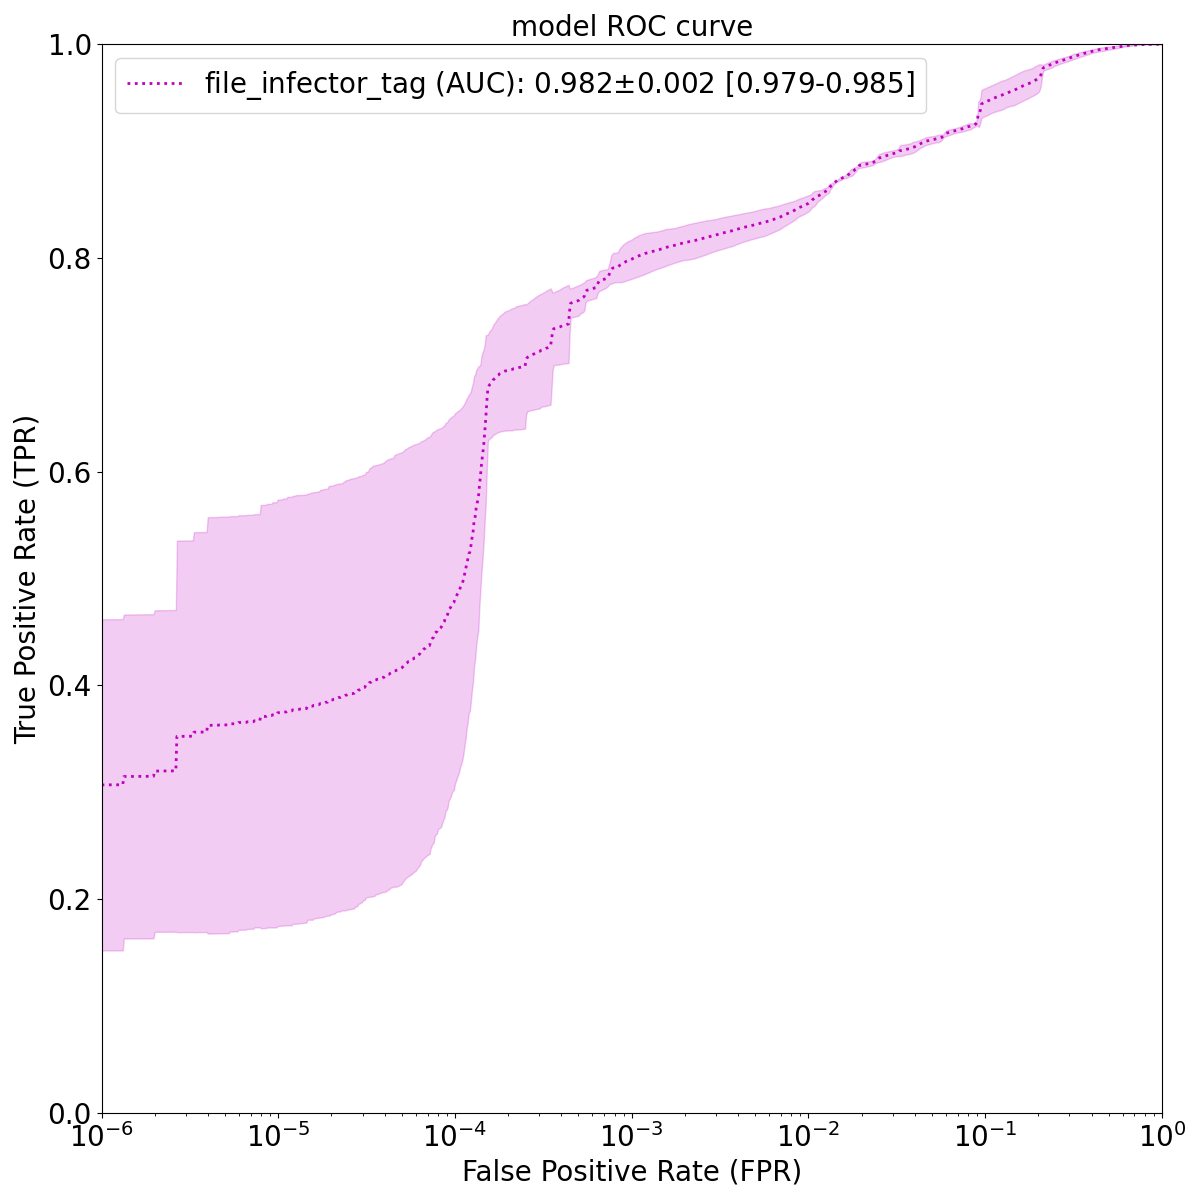
\includegraphics[width=0.6\textwidth]{./results/file_infector_tag_roc_aloha.png}
        \vspace*{-0.2cm}
        \caption{ROC curve and AUC statistics of \textBF{ALOHA} model for the \textbf{File-infector Tag}. The line represents the \textit{mean} TPR at a given FPR, while the shaded region represents the \textit{standard deviation}. Statistics were computed over \textBF{3} training runs, each with random parameter initialization.}
        \label{fig:fileInfectorTagRocAloha}
    \end{figure}
}

\newcommand{\fileInfectorTagRocJointEmbedding}{
    \begin{figure}[H]
        \vspace*{-0.5cm}
        \centering
        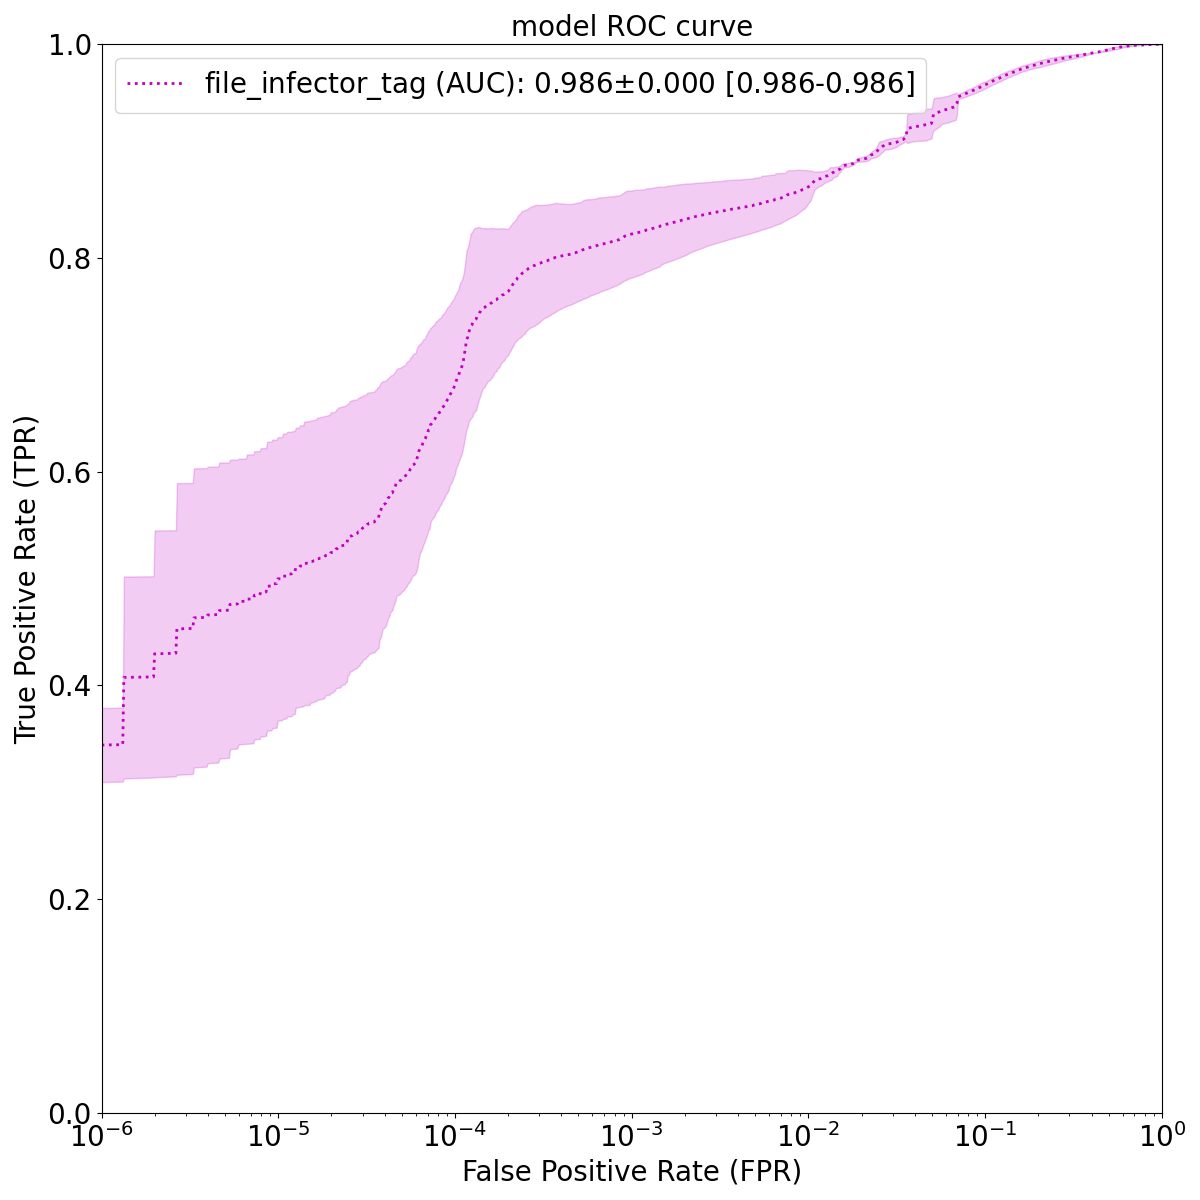
\includegraphics[width=0.6\textwidth]{./results/file_infector_tag_roc_jointEmbedding.png}
        \vspace*{-0.2cm}
        \caption{ROC curve and AUC statistics of \textBF{Joint Embedding} model for the \textbf{File-infector Tag}. The line represents the \textit{mean} TPR at a given FPR, while the shaded region represents the \textit{standard deviation}. Statistics were computed over \textBF{3} training runs, each with random parameter initialization.}
        \label{fig:fileInfectorTagRocJointEmbedding}
    \end{figure}
}

\newcommand{\fileInfectorTagRocProposedMethod}{
    \begin{figure}[H]
        \vspace*{-0.5cm}
        \centering
        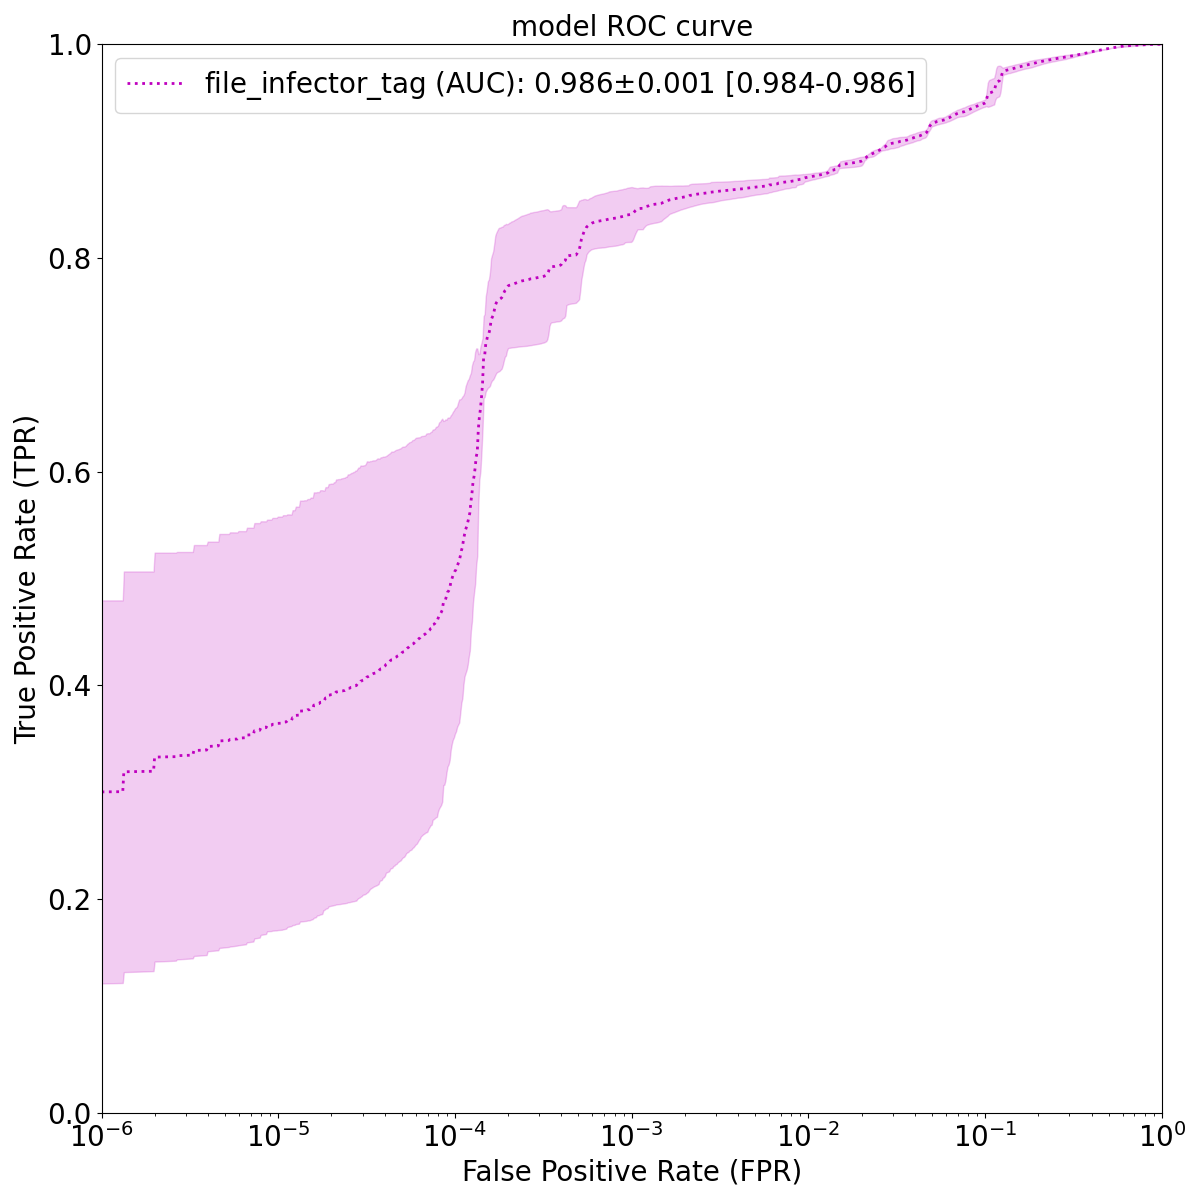
\includegraphics[width=0.6\textwidth]{./results/file_infector_tag_roc_proposedModel.png}
        \vspace*{-0.2cm}
        \caption{ROC curve and AUC statistics of \textBF{Proposed Model} for the \textbf{File-infector Tag}. The line represents the \textit{mean} TPR at a given FPR, while the shaded region represents the \textit{standard deviation}. Statistics were computed over \textBF{3} training runs, each with random parameter initialization.}
        \label{fig:fileInfectorTagRocProposedModel}
    \end{figure}
}
